\documentclass[10pt,a4paper]{article}
\usepackage[pdftex]{graphicx}
\usepackage{graphicx}
\usepackage{amsmath}
\usepackage{listings}
\usepackage{url}
\usepackage{amsmath}
\usepackage[left=20mm, top=0in]{geometry}
\usepackage[utf8]{inputenc}
\date{}
\begin{document}
\title{Assignment No 8: THE DIGITAL FOURIER TRANSFORM}
\author{JAGAN M J EE20B047}
\maketitle


\section{AIM}

Aim is to examine the DFT of various functions using the fft library in numpy

\section{THE SINUSOIDS}
The DFT of sinusoidal function: \\

\begin{equation*}
 y = \ \sin(x) \ = \frac{e^{jx} - e^{-jx}}{2j} 
\end{equation*}
is given by :\\
\begin{equation*}
Y(\omega) = \frac{\delta (\omega - 1) - \delta (\omega + 1)}{2j}
\end{equation*}

We plot the spectrum of sin(5t) and also its phase and is as shown below: \\\\\\\\\\\\\\

\begin{figure}[!tbh]

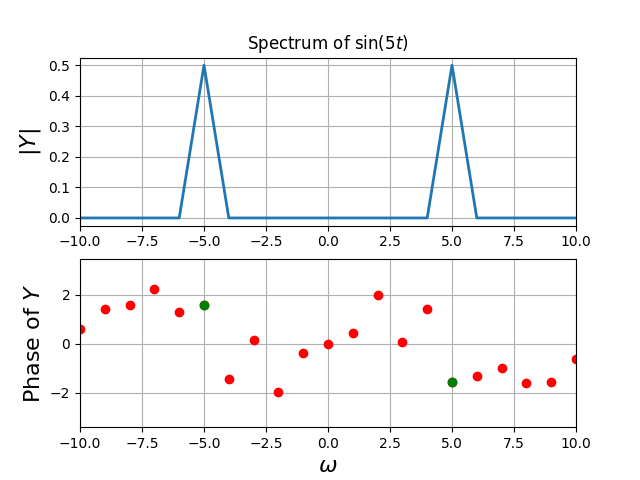
\includegraphics[width = 0.9\textwidth]{1- spectrum of sin(5t) [with NO errors in plot].png}
\caption{Spectrum and Phase plots of sin(5t)}

\end{figure}

We also plot the spectrum of (1+0.1cos(t))cos(10t) and also its phase and is as shown below:

\begin{figure}[!tbh]

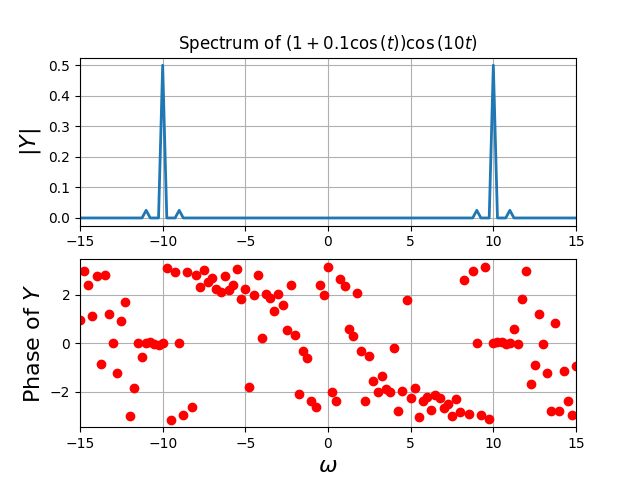
\includegraphics[width = 0.9\textwidth]{1-spectrum of AM wave (high no of samples).png}
\caption{Spectrum and Phase plots of (1+0.1cos(t))cos(10t)}

\end{figure}

\section{Spectrum of $\sin^{3} t$ and $\cos^{3} t$}

We know \\ 

\begin{equation*}
 \\sin^{3} t = \frac{3\\sin t}{4} - \frac{\\sin 3t}{4}
\end{equation*}

and its Fourier transform is given by : \\

\begin{equation*}
F(\\sin^{3} t) = \frac{3}{8j}(\delta (\omega - 1) - \delta (\omega + 1)) - \frac{1}{8j}(\delta (\omega - 3) - \delta (\omega + 3))
\end{equation*} 

Also 

\begin{equation*}
 \\cos^{3} t = \frac{3\\cos t}{4} + \frac{\\cos 3t}{4}
\end{equation*}

and its Fourier transform is given by : \\

\begin{equation*}
F(\\cos^{3} t) = \frac{3}{8j}(\delta (\omega - 1) + \delta (\omega + 1)) + \frac{1}{8j}(\delta (\omega - 3) + \delta (\omega + 3))
\end{equation*} 

We plot the spectrum of $\sin^{3} t$ and is as shown below:\\\\\\\\\\\\\\\\\\

\begin{figure}[!tbh]

\includegraphics[width = 0.9\textwidth]{2-spectrum of sin³(t).png}
\caption{Spectrum of $\sin^{3} t$}

\end{figure}

We also plot the spectrum of $\cos^{3} t$ and is as shown below:\\\\\\\\\\\\\\\\\\\\\\\\\\\\\\\\\\\\\\\\\\\\\\\\\\\\\\\\

\begin{figure}[!tbh]

\includegraphics[width = 0.9\textwidth]{2-spectrum of cos³(t).png}
\caption{Spectrum of $\cos^{3} t$}

\end{figure}










\section{Spectrum of $\cos( 20t + 5\cos t)$}

The following plot shows the DFT of the function and also its phase where the magnitude is greater than 0.001 : 

\begin{figure}[!tbh]

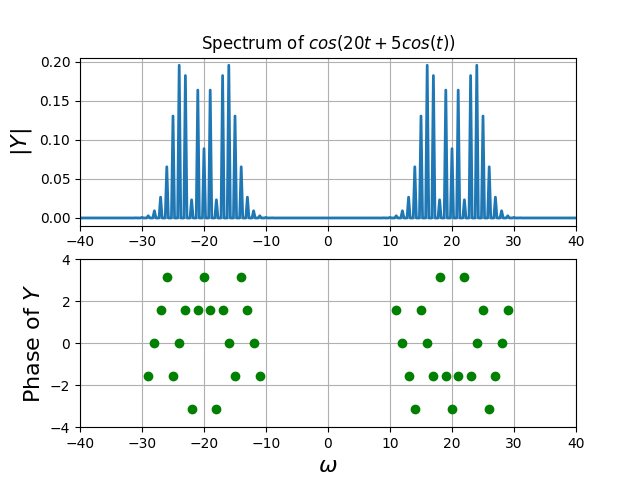
\includegraphics[width = 0.9\textwidth]{3-spectrum of cos(20t +5 cos(t)).png}
\caption{Spectrum of $\cos( 20t + 5\cos t)$}

\end{figure}

Clearly the carrier frequency is 20 and this signal is a frequency modulated function. So mainly there are impulses at the carrier frequecy and also at side band frequencies that are clsoe to the carrier frequency and later decays on either side.


\section{DFT of a Gaussian}

 DFT of Gaussian $e^{-t^2/2}$ is given by : 

\begin{equation*}
F(e^{-t^2/2}) = \frac{e^{-\omega^2/2}}{\sqrt{2\pi}}
\end{equation*}

We plot the DFT of the gaussian and is as shown below : 

\begin{figure}[!tbh]

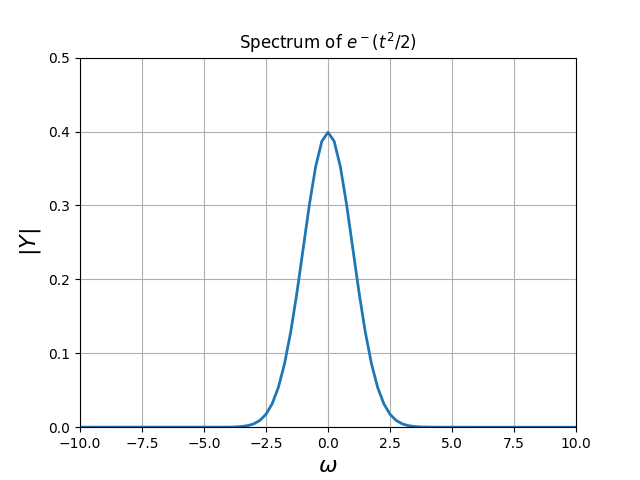
\includegraphics[width = 0.9\textwidth]{4- spectrum of gaussian.png}
\caption{Spectrum of a gaussian function}

\end{figure}

Also efforts are made in order to find the error produced between the actual DFT and the DFT that we obtained by setting a tolerance of $10^{-15}$ and also finding the most suitable time range that is so accurate. The error is computed for each time range and the time range gets updated to twice its value for the computation of the succeeding error and the loop stops when the error is less than the given tolerance, say $10^{-15}$ \\

Accuracy of DFT : 1.337286e-17\\
Most suitable time range : [$-4\pi, 4\pi$], as T is obtained as 25.1327 equal to $8\pi$


\section{Conclusion}

We analysed on how to find DFT for various types of signals and minimizing the error with tolerance upto $10^{-15}$ . We used fast fourier transform method to compute DFT. We have used FFT for signals with samples in $2^{k}$ as it works well this sampling.

\end{document}